\acresetall
\chapter{Introduction}
\label{chapter:introduction}

The \ac{waas} is a navigational aid developed by the \ac{faa} with the goal of providing improved accuracy, integrity and availability of the \ac{gps} giving aviation users the ability to use \ac{gps} in all phases of flight.  The purpose of this sensitivity analysis is to isolate the performance of the \ac{ccc} integrity monitor and show the gains made to reduce its bounding variance so that an increase in availability is attained while integrity is maintained. The purpose of the \ac{ccc} monitor is to detect satellite failures that cause the code phase and carrier phase of \ac{gps} to be incoherent.  Within \ac{waas} and the end user equipment there is an assumption that the code and carrier are coherent, but there has never been an empirical analysis of its performance.  To understand the complexities of why this has never been done additional details about the \ac{waas} architecture are required.

\begin{figure}
	\centering
	\scalebox{.35}{
	\mbox{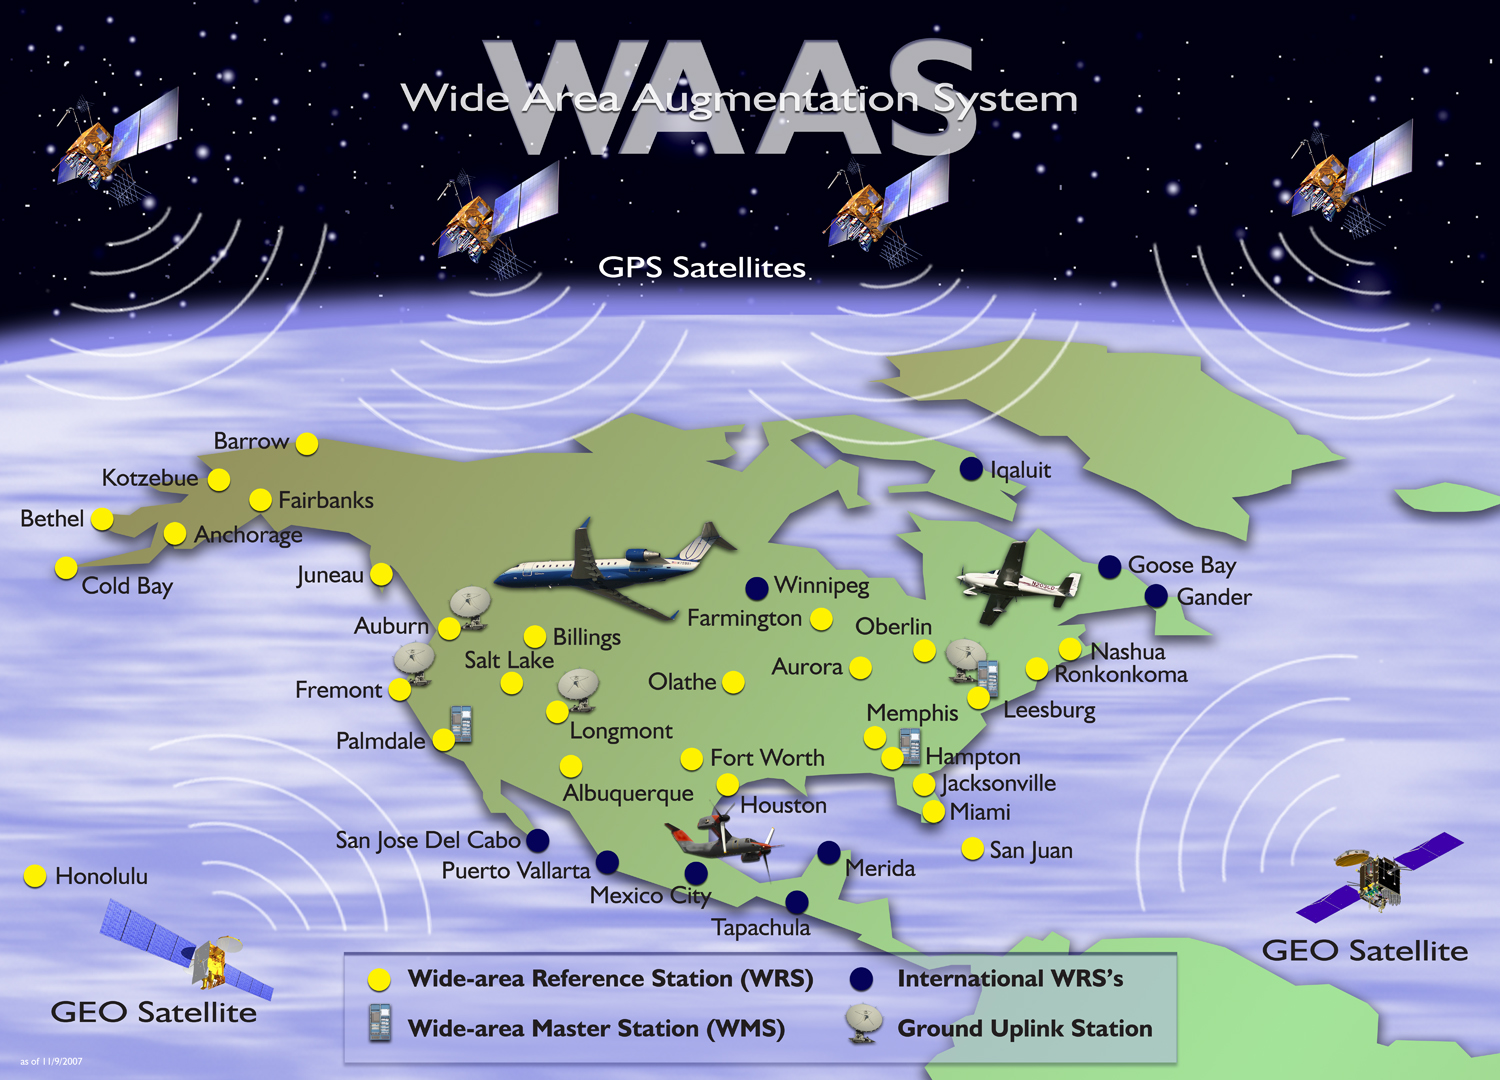
\includegraphics{figures/waas-overview-1.jpg}}
	}
	\caption{The Wide Area Augmentation System}
	\label{fig:WAAS-Overview-1}
\end{figure}

The stated goal of \ac{waas}, to provide improve accuracy, integrity and availability, is accomplished in the following ways: accuracy is improved by providing a differential \ac{gps} solution. The \ac{waas} architecture is a geographically diverse sensor network of high fidelity \ac{gps} receivers that track \ac{gps} satellites throughout North and Central America and Hawaii. This network consists of 114 \ac{gps} receivers at 38 geographically diverse sites.  Any error in time translates directly into an error in the range measurement to the \ac{gps} satellite, so to provide the highest degree of accuracy the \ac{gps} antennas are designed to mitigate multipath and each \ac{gps} receiver clock is disciplined with a cesium frequency standard to provide a highly accurate and precise time source. A quarterly analysis of every second of every day is performed to observe if any change in the environment has occurred that may negatively affect performance. Yearly releases are conducted to update the antenna positions so that continental drift and other environmental factors are mitigated. The rigor put into this infrastructure enables this highly precise network of receivers to detect errors within \ac{gps} and the geographic diversity enables modeling of delays in the ionosphere. Once an end user within the \ac{waas} coverage area applies the \ac{gps} and ionospheric corrections they can attain sub-meter level \ac{gps} accuracy in the best case and maximums still under 2 meters in the worst case. There are more than a dozen safety integrity monitors built into \ac{waas} that monitor \ac{gps} and ionospheric threats. Protecting users from integrity threats is an integral part of \ac{waas} as it was commissioned as a safety-of-life system, but integrity and availability have to be considered together as there is an inverse relationship between the two. As integrity increases availability is reduced. All \ac{gps} threats would be abated if \ac{gps} were not allowed to be used; integrity against \ac{gps} threats is 100\% while utilization of \ac{gps} is 0\%.  To achieve an acceptable level of utilization of \ac{gps} availability, confidence bounding is performed for \ac{gps} and ionospheric threats. The purpose of this study is to isolate the performance of the \ac{ccc} integrity monitor and show the gains made to reduce its bounding variance so that an increase in availability is attained while integrity is maintained.

The cost of establishing and maintaining a high fidelity \ac{gps} monitoring network is considerable. Establishing the infrastructure and algorithms for the \ac{ioc} of \ac{waas} cost the United States government over \$4 Billion and the yearly maintenance cost are approximately \$100 million per year. Costs of this level prohibit all but a few countries from establishing a monitoring system of this magnitude. Further attaining access to the data along with the infrastructure to store and analyze the data is cost prohibitive. Over my tenure at the \ac{faa} there has been a concerted effort to establish the capability to perform an analysis of this extent. The infrastructure for collecting, storing and analyzing data at this volume has cost over \$5 million to establish and has pushed the limits of hardware and software.

Though there was considerable time, effort and funding in establishing the capability outlined in this study, the approach in this study utilizes commodity hardware and open source databases, programming languages and analytics software. Further this capability was established to analyze as very specific data set. For the range measurements alone there are $\approx$374,284,800 data points per day.  The equipment required to process this was scaled commensurately for the data that is collected each day times the 7 years of data collected. Over 950 billion data points for just a single type of measurement and several hundred data elements are stored. The approach utilized in this study can be scaled appropriately to the application domain so cost for establishing a similar capability is tenable.

The approach outlined in this analysis is innovative in that it can be utilized to increase the availability of any Space Based Augmentation System while maintaining integrity.  This infrastructure is limited to all but a few countries, but with the countries that are developing this capability, world wide space based augmentation can be attained. The application of this methodology could lead to the establishment of highly available space based navigational aids on a global level. Further. the generalized approach utilized to solve this big data analytics problems can be utilized in domains outside of this specific aviation application.

Global SBAS Picture

\href{https://www.gps.gov/policy/funding/2017/}{https://www.gps.gov/policy/funding/2017/}

\href{http://commdocs.house.gov/committees/Trans/hpw106-100.000/hpw106-100\_1.HTM}{http://commdocs.house.gov/committees/Trans/hpw106-100.000/hpw106-100\_1.HTM}

\href{https://www.gps.gov/technical/ps/2008-waas-performance-standard.pdf}{https://www.gps.gov/technical/ps/2008-waas-performance-standard.pdf}

Things I need.

PRN SVN Mapping for the last five years.
Assign to Hoang.


First sentence what this dissertation has achieved.
30,000ft view of \ac{waas} and the Problem. Pros and Cons of \ac{waas} and the specific area I am looking at.

Paragraph 1: What is the problem?

Not more than 3-4 sentences telling the reader what the problem is, in as simple English as possible

Paragraph 2: Why is the problem hard?

What has eluded us in solving it? What does the literature say about this problem? What are the obstacles/challenges? Why is it non-trivial?

Paragraph 3: What is your approach/result to solving this problem?

How come you solved it? Think of this as your “startling” or “sit up and take notice” claims that your dissertation will plan to prove/demonstrate

Paragraph 4: What is the consequence of your approach?

So, now that you’ve made me sit up and take notice, what is the impact? What does your approach/result enable?
~\\

\ac{waas} has $\approx$2000 \ac{osp} values that define minimum and maximum limits, action thresholds, and timeouts. The parameters are use to control logic throughout the \ac{waas} system. There is always a balance between usability and safety.  For the \ac{faa} these are in the terms availability/continuity for usability and integrity for safety.  If the system remains off then this is the highest level of integrity, meaning if the user does not use the \ac{gps} then they are safe against all \ac{gps} related threats.  This would not make a practical system, so it led the engineers developing the \ac{waas} application to use values that would allow the system to be usable, but were significantly conservative to protect the user against \ac{gps} related threats.  At the inception of \ac{waas} there was insufficient empirical data to appropriately set many of the integrity bounding limits.  At least one value was stated as being grossly overbounded and that the empirical evidence to set it correctly would require many years of data.  The \ac{nase} organization has now accumulated the several years of data, but there is currently no analytical system in place to process this volume of data so that updated \ac{osp} values can be set.

Currently in this research effort the beginnings of a system have been created that can be used as an analytics platform for getting the varying data formats and elements into a common format where meaningful analysis can be performed.  Every component in the system is purposely selected or designed to take data from its rawest form and process it into a format that can be utilized, manipulated and assessed. As of this writing the system can process NovAtel GUST, G-II and G-III \ac{gps} receiver binary log files. The software can identify receiver log messages, \ac{crc} check that the messages is valid and break each message type into its constituent elements for storing and further analysis. This has been fully demonstrated end to end on a \ac{geo} Satellite monitoring system in development. This system is currently monitoring one \ac{geo} satellite at one \ac{gus} site but will be expanded to four \ac{geo}s at 8 \ac{gus} sites in the near future. It process data from the \ac{waas} application receiver and a second receiver used for fault isolation. The system is logging $\approx$1213 data elements per second from only two message types and this number will grow as more message types are recorded to the database.
